\section{Iterazione 2}

\subsection{Introduzione}
Nella seconda iterazione si è deciso di implementare i seguenti casi d'uso:

\begin{itemize}
    \item UC6 Gestioni prenotazioni \textit{[Astratto]}
    \begin{itemize}
        \item UC6.1 Nuova prenotazione
        \item UC6.2 Visualizzazione prenotazioni
    \end{itemize}
    \item UC7 Algoritmo gestione barche ed escursioni
\end{itemize}

\subsection{UC6: Gestione prenotazioni}
\emph{Breve descrizione}: L'utente, dopo essersi loggato, può effettuare la prenotazione per una delle escursioni organizzate dal proprietario. É possibile prenotare un posto non solo per sé stesso ma anche per altre persone, indicando il numero di partecipanti totale. Oltre alla creazione di una prenotazione, l'utente deve poter visualizzare le prenotazioni effettuate.
Il caso d'uso \textit{Gestione prenotazioni} è suddiviso in 2 casi d'uso concreti:

\begin{itemize}
    \item UC6.1 Nuova prenotazione
    \item UC6.2 Visualizzazione prenotazioni 
\end{itemize}

\subsubsection{UC6.1 Nuova prenotazione}
 \emph{Breve descrizione}: L'utente effettua una nuova prenotazione per un'escursione organizzata dal proprietario.\medbreak
 \emph{Attori coinvolti}: Utente, Sistema.\medbreak
 \emph{Trigger}: L'utente clicca il bottone \textit{Book excursion}.\medbreak
 \emph{Postcondizione}: Il sistema mostra la nuova prenotazione all'interno della pagina di visualizzazione delle prenotazioni.\medbreak
 \emph{Procedimento}:

\begin{enumerate}
    \item L'utente si trova sulla \textit{User page} e clicca il bottone \textit{Book excursion}.
    \item Il sistema mostra un calendario.
    \item L'utente seleziona la data desiderata.
    \item Il sistema mostra una lista degli orari disponibili per quella data, se presenti.
    \item L'utente seleziona l'orario desiderato e inserisce il numero di partecipanti all'escursione. Infine, clicca il bottone \textit{Book}.
    \item Il sistema utilizza l'algoritmo (si veda il paragrafo \ref{algoritmo}) che permette di allocare in modo efficiente il gruppo alle barche disponibili per l'escursione scelta. Successivamente mostra un messaggio per notificare l'avvenuta o mancata prenotazione dell'escursione.
    \item In caso di prenotazione a buon fine, il sistema mostra la prenotazione effettuata nella pagina di visualizzazione delle prenotazioni \textit{My excursions}.
\end{enumerate}

\subsubsection{UC6.2 Visualizzazione prenotazioni}
 \emph{Breve descrizione}: L'utente visualizza le prenotazioni effettuate e i relativi dati.\medbreak
 \emph{Attori coinvolti}: Utente, Sistema.\medbreak
 \emph{Trigger}: L'utente clicca il bottone \textit{My excursions}. \medbreak
 \emph{Postcondizione}: Il sistema mostra una vista con l'elenco delle prenotazioni.\medbreak
 \emph{Procedimento}:

\begin{enumerate}
    \item L'utente effettua il login
    \item L'utente clicca il bottone \textit{My excursions} presente nella \textit{User page}.
    \item Il sistema mostra l'elenco delle prenotazioni presenti nel database a nome dell'utente con le seguenti informazioni:
    \begin{itemize}
        \item Data e ora escursione
        \item Numero di persone per cui è stata prenotata l'escursione
    \end{itemize}
\end{enumerate}

\clearpage
\subsection{UC7: Algoritmo barche ed escursioni}\label{algoritmo}
 \emph{Breve descrizione}: L'utente richiede di effettuare una prenotazione per un'escursione specificando data, orario e numero di persone del gruppo. Il sistema deve allocare il gruppo in modo ottimale, tenendo conto dei posti rimanenti sulle barche. Lo scopo principale dell'algoritmo è quello di minimizzare il numero di barche impiegate per l'escursione, in modo da ridurre i costi del proprietario. Per massimizzare il numero di prenotazioni, se il gruppo è troppo grande per i posti rimanenti sulle barche, si cerca di dividere il gruppo in due e allocarlo su due barche. Nel caso in cui non fosse possibile l'allocazione in questo modo, la prenotazione non può essere effettuata. L'algoritmo è quindi di tipo greedy. \medbreak
 \emph{Attori coinvolti}: Sistema.\medbreak
 \emph{Trigger}: L'utente richiede di effettuare una prenotazione.\medbreak
 \emph{Postcondizione}: Prenotazione effettuata o fallita.\medbreak
 \emph{Passi dell'algoritmo}:

\begin{enumerate}
    \item Il primo passo dell'algoritmo viene attivato dal tentativo di prenotazione di un'escursione da parte di un utente per un gruppo di \textbf{N} persone.
    \item Viene calcolato il numero di posti rimanenti (\textbf{P}) sulle barche per l'escursione scelta.
    \begin{enumerate}
        \item se P > 0, l'algoritmo procede con il passo successivo.
        \item se P <= 0, l'algoritmo termina con il \textbf{fallimento} della prenotazione, in quanto per l'escursione scelta non sono presenti posti rimanenti. 
    \end{enumerate}
    \item Si cerca una barca per cui sono stati già allocati altri gruppi, in modo tale da cercare di minimizzare il numero di barche utilizzate per escursione. La barca deve avere abbastanza posti rimanenti (\textbf{PR}) per contenere il gruppo per cui l'utente ha prenotato, ovvero deve verificarsi PR >= N. La ricerca ritorna una lista di barche.
    \begin{enumerate}
        \item Se la lista è vuota, si procede con il passo successivo.
        \item \label{ordinamento} Se la lista non è vuota, essa viene ordinata in ordine crescente di posti rimanenti. Infine viene scelta la prima barca della lista, ovvero la barca che ha il numero minimo di posti rimanenti. La prenotazione termina con \textbf{successo}. 
    \end{enumerate}
    \item Si cerca una barca vuota (con capienza \textbf{C}), ovvero per cui non è stato già allocato alcun gruppo per l'escursione selezionata dall'utente. La barca deve poter contenere il gruppo, ovvero deve verificarsi C >= N. La ricerca ritorna una lista di barche. 
    \begin{itemize}
        \item Se la lista è vuota, si procede con il passo successivo.
        \item Se la lista non è vuota, si procede come al punto \ref{ordinamento}. La prenotazione quindi termina con \textbf{successo}.
    \end{itemize}
    \item Arrivati a questo passo dell'algoritmo, significa che il gruppo non può essere allocato per intero né su un barca vuota, né su una barca in cui sono già presenti altri gruppi per l'escursione scelta. La scelta è stata di cercare di allocare il gruppo dividendolo in due gruppi separati solo se composto da un numero di persone superiore ad una soglia minima. In caso contrario c'è il \textbf{fallimento} della prenotazione. Si cercano quindi due barche (vuote o già parzialmente occupate) con PR >= N/2. In caso di gruppi dispari una barca deve avere PR >= N/2, l'altra PR >= (N/2)+1. La ricerca ritorna una lista di barche.
    \begin{enumerate}
        \item Se esistono due barche in grado di contenere il gruppo diviso, si procede come al punto \ref{ordinamento} e la prenotazione termina con \textbf{successo}.
        \item In caso contrario, neanche dividendo il gruppo è possibile trovare abbastanza posti, quindi si ha il \textbf{fallimento} del tentativo di prenotazione da parte dell'utente. 
    \end{enumerate}
\end{enumerate}

In Figura \ref{fig:pseudocodice1} e \ref{fig:pseudocodice2} viene mostrato lo pseudocodice dell'algoritmo con l'analisi di complessità. Nell'eseguire l'analisi di complessità si considera il numero di barche pari al valore \textit{n} e il numero di prenotazioni pari al valore \textit{m}. La complessità dell'algoritmo è scritta nell'equazione \ref{complessità}. 
\begin{equation}
O(\max{(m,\log{n})})
\label{complessità}
\end{equation}

\begin{figure}[htbp]
    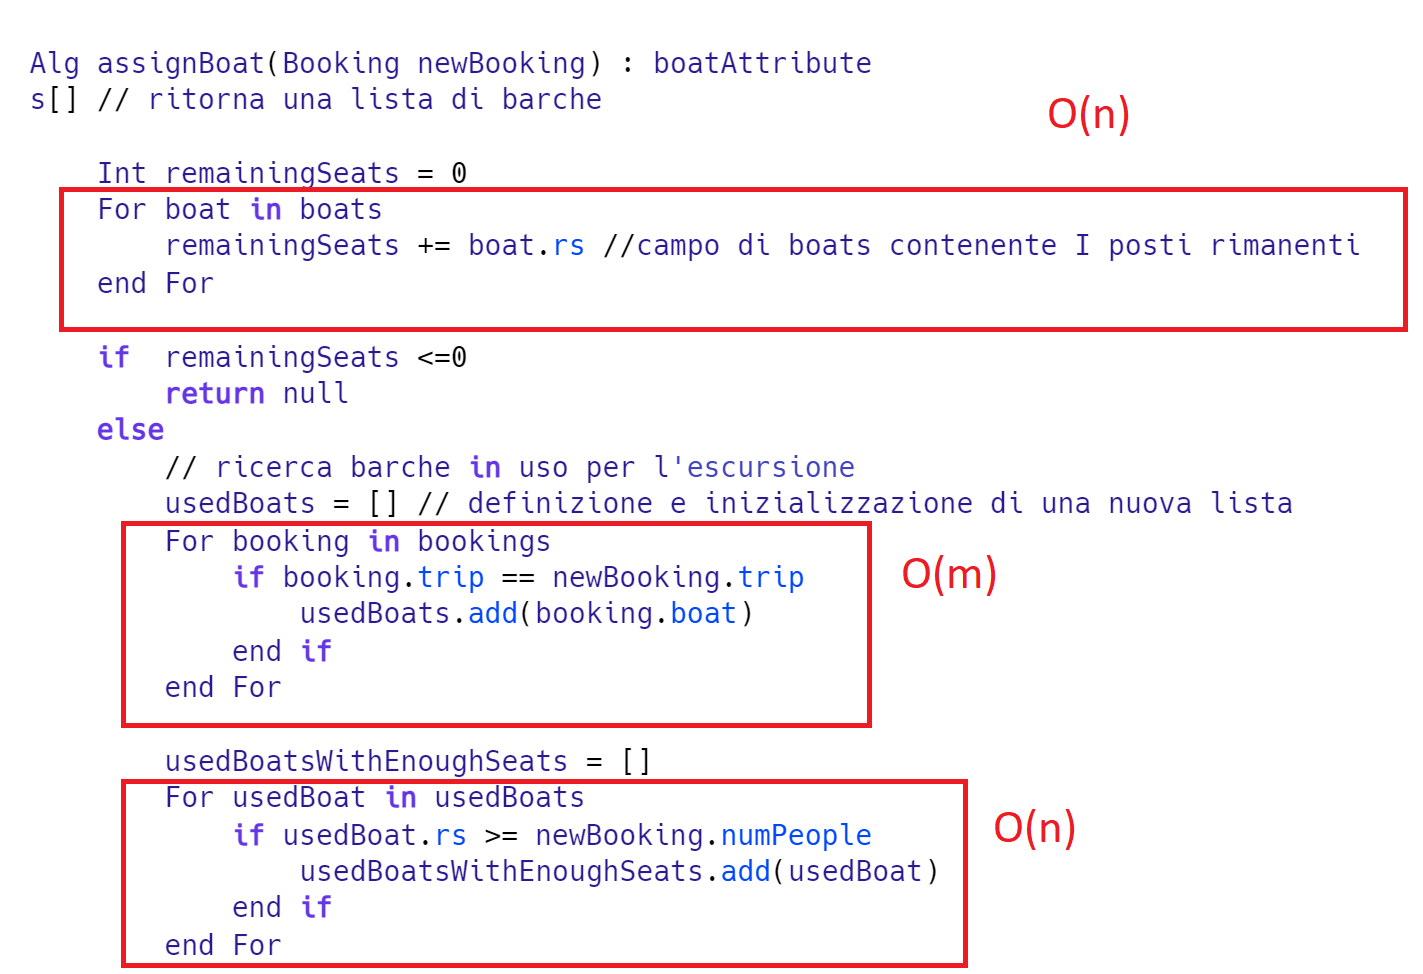
\includegraphics[scale=0.5]{images/iterazione2/pseudocodice/1.png}
    \centering
    \caption{Pseudocodice algoritmo - Parte 1}
    \label{fig:pseudocodice1}
\end{figure}
\begin{figure}[htbp]
    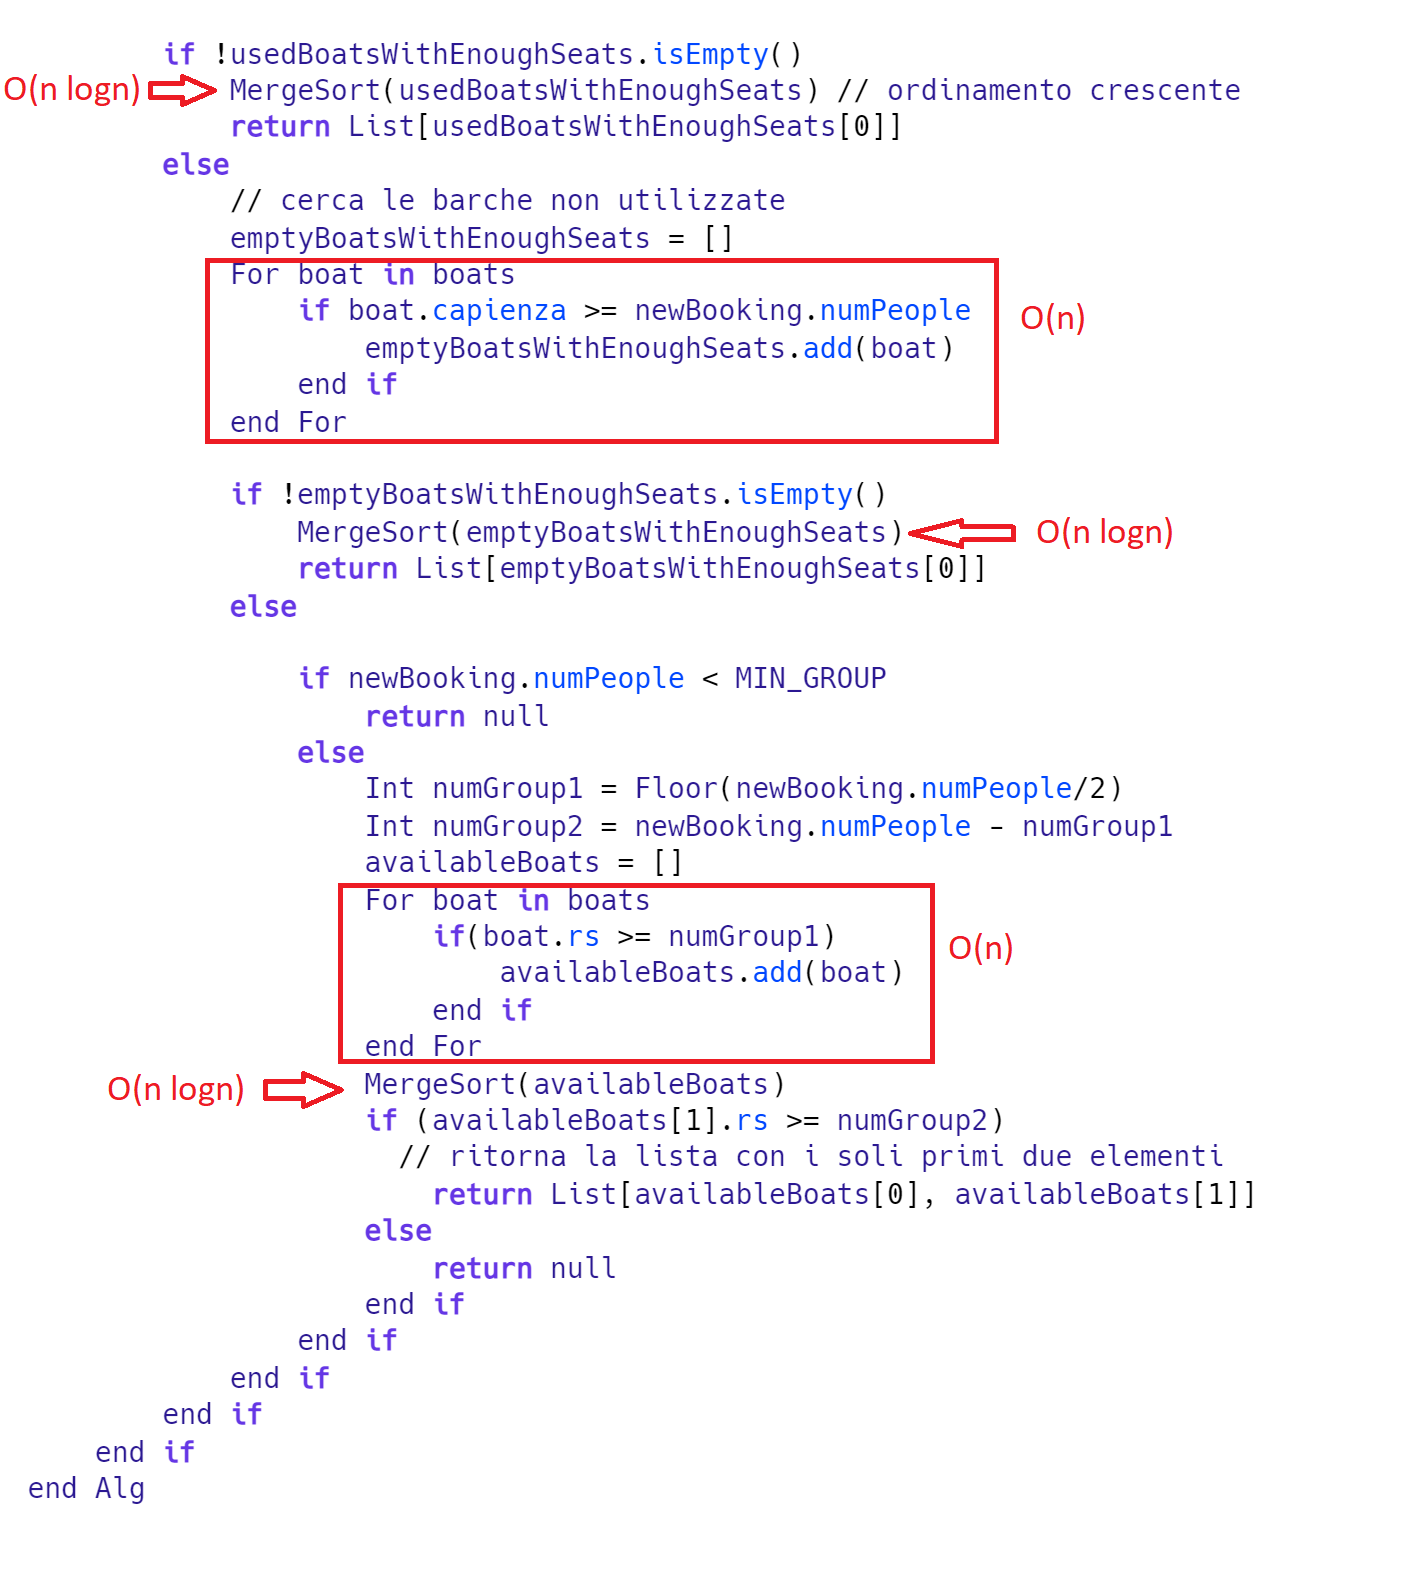
\includegraphics[scale=0.5]{images/iterazione2/pseudocodice/2.png}
    \centering
    \caption{Pseudocodice algoritmo - Parte 2}
    \label{fig:pseudocodice2}
\end{figure}

\begin{figure}[htbp]
    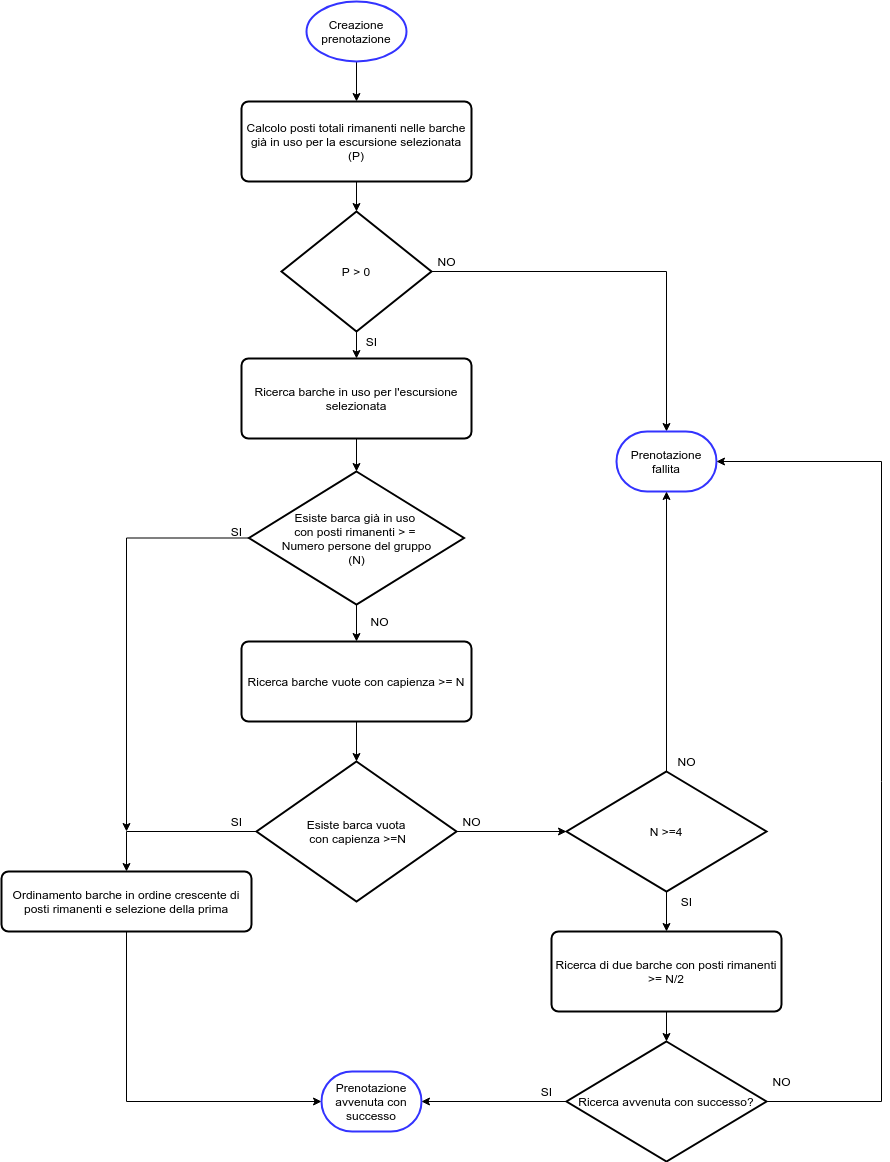
\includegraphics[scale=0.45]{images/iterazione2/flowChart.png}
    \centering
    \caption{Flow chart dell'algoritmo}\label{fig:flowChart}
\end{figure}

\clearpage
\subsection{UML Component Diagram}
I casi d’uso scelti nella seconda iterazione vengono aggiunti al \textit{Component Diagram} dell'iterazione 1 (Figura \ref{fig:componentDiagram}). Il nuovo diagramma viene mostrato in  Figura~\ref{fig:componentDiagram2}.

\begin{figure}[htbp]
    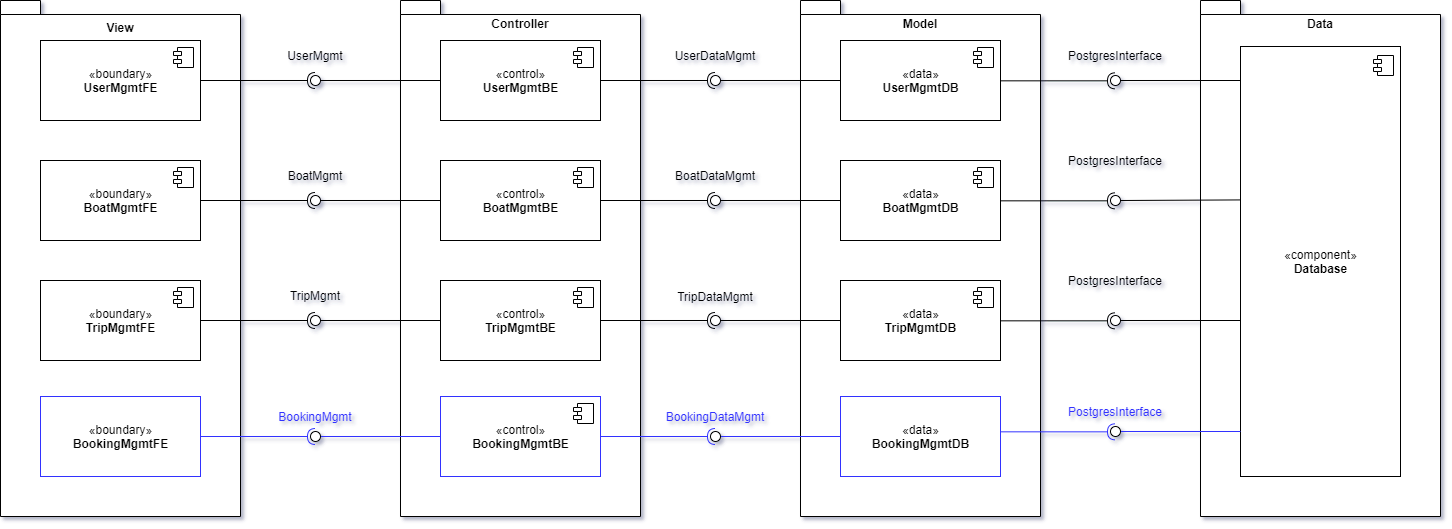
\includegraphics[width=\textwidth]{images/iterazione2/diagrams/ComponentDiagram_v1.png}
    \centering
    \caption{UML Component Diagram}\label{fig:componentDiagram2}
\end{figure}

\clearpage
\subsection{UML Class Diagram per interfacce}
Il diagramma in Figura~\ref{fig:ClassDiagramInterfaces2} mostra le interfacce relative ai nuovi casi d'uso.

\begin{figure}[htbp]
    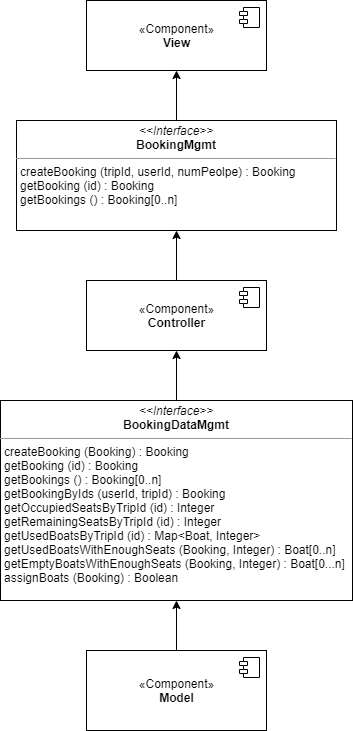
\includegraphics[scale=0.5]{iterazione2/diagrams/ClassDiagramInterfaces_v1.png}
    \centering
    \caption{UML Class Diagram per interfacce}
    \label{fig:ClassDiagramInterfaces2}
\end{figure}

\clearpage

\subsection{UML Class Diagram per tipi di dato}
Il tipo di dato \textit{Booking} introdotto in questa iterazione, viene inserito nel \textit{Class Diagram per tipo di dato} (vedi Figura \ref{fig:ClassDiagramTypes}) dell'iterazione precedente. Il nuovo diagramma, mostrato in Figura~\ref{fig:ClassDiagramTypes2}, mostra anche le relazioni tra i tipi di dato instauratesi grazie all'aggiunta del nuovo tipo di dato. 

\begin{figure}[htbp]
    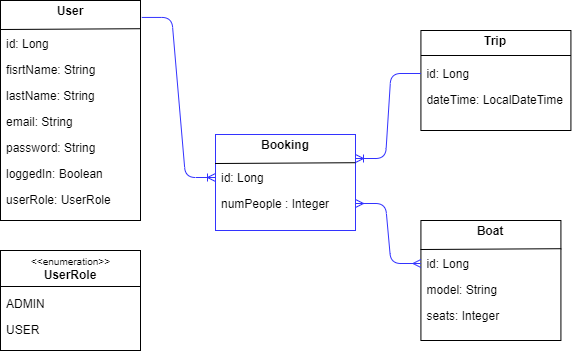
\includegraphics[width=\textwidth]{iterazione2/diagrams/ClassDiagramTypes_v1.png}
    \centering
    \caption{UML Class Diagram per tipi di dato}
    \label{fig:ClassDiagramTypes2}
\end{figure}

\clearpage
\subsection{UML Deployment Diagram}
I nuovi componenti relativi all'iterazione 2 vengono inseriti nel \textit{Deployment Diagram} dell'iterazione precedente (vedi Figura \ref{fig:DeploymentDiagram}). Il nuovo diagramma è mostrato in Figura~\ref{fig:DeploymentDiagram2}.

\begin{figure}[htbp]
    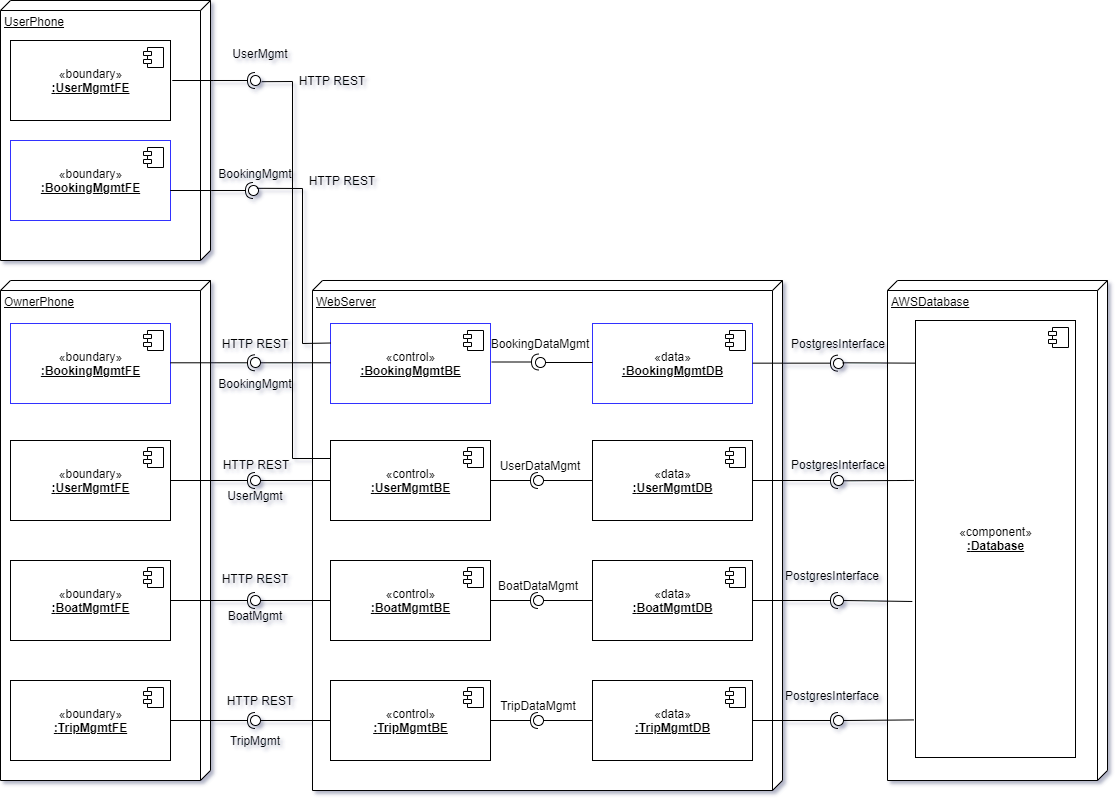
\includegraphics[width=\textwidth]{iterazione2/diagrams/DeploymentDiagram_v1.png}
    \centering
    \caption{UML Deployment Diagram}\label{fig:DeploymentDiagram2}
\end{figure}

\clearpage
\subsection{Testing}

\subsubsection{Analisi statica}
Come visto nel paragrafo \ref{analisi-statica} è stata utilizzata l'estensione \textit{Language Support for Java(TM) by Red Hat} fornita
dall'IDE \textit{Visual Studio Code}.

\subsubsection{Analisi dinamica}
Per l'iterazione 2 è stato effettuato il test delle seguenti funzioni:
\begin{itemize}
  \item Creazione prenotazione a buon fine
  \item Creazione prenotazione errata
  \item Visualizzazione prenotazione a buon fine
\end{itemize}

I risultati sono riportati in Figura \ref{Risultati test dinamico iterazione 2}. 

\begin{figure}[htbp]
    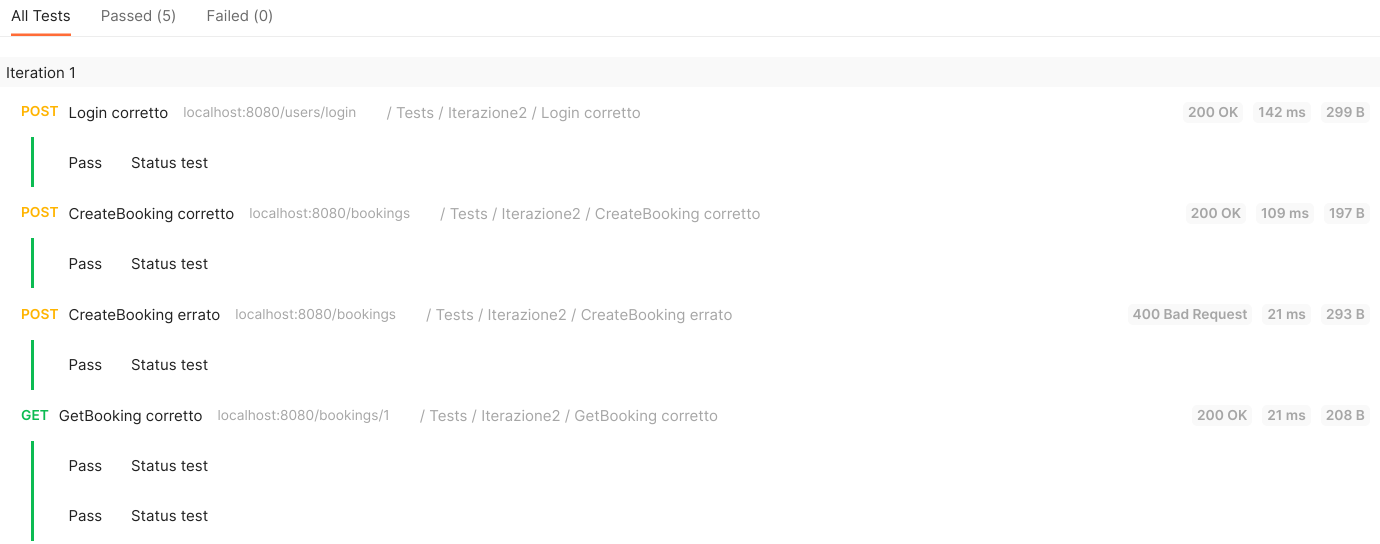
\includegraphics[width=\textwidth]{iterazione2/test/service-test.png}
    \centering
    \caption{Risultati test dinamico}
    \label{Risultati test dinamico iterazione 2}
\end{figure}

\subsubsection{Unit Test}
Per questa iterazione è stata testata la funzione \textit{findByTripId} che serve per filtrare le prenotazioni e ottenere solo quelle relative ad una certa data.

\clearpage

\begin{lstlisting}[language=Java]
@DataJpaTest
class BookingRepositoryTest {

    @Autowired
    private BookingRepository underTest;

    @Autowired
    private UserRepository userRepository;

    @Autowired
    private BoatRepository boatRepository;

    @Autowired
    private TripRepository tripRepository;

    @Test
    void findByTripIdOk() {
        // given
        User user = new User("Marco", "Bisceglia", 
        "marco@gmail.com", "marco", "MMM");
        userRepository.save(user);

        Boat boat = new Boat("B1", 4);
        boatRepository.save(boat);

        LocalDateTime dayTrip = LocalDateTime.of
        (2022, Month.JANUARY, 01, 10, 00, 00);
        Trip trip = new Trip(dayTrip);
        tripRepository.save(trip);

        Booking expected = new Booking(5);
        expected.setUser(user);
        expected.setBoat(boat);
        expected.setTrip(trip);
        underTest.save(expected);

        // when
        List<Booking> result = underTest.findByTripId(1L);

        // then
        assertThat(expected).isEqualTo(result.get(0));
    }
}
\end{lstlisting}

Il test ha confermato la correttezza della funzione. 

\begin{figure}[htbp]
    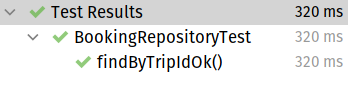
\includegraphics[width=\textwidth]{iterazione2/test/unit-test.png}
    \centering
    \caption{Risultato Unit Test}
    \label{test Junit findByTripId}
\end{figure}

\clearpage

\subsubsection{Integration Test dell'algoritmo}
L'algoritmo che alloca i gruppi di persone sulle barche disponibili, per poter funzionare, necessita di funzioni presenti in moduli differenti: barche, utenti, escursioni e prenotazioni. Non è quindi possibile realizzare un test di unità che testa la singola funzione; si realizza invece un test di integrazione.
A tal scopo è stato realizzato uno script in Python durante la fase di programmazione dell'algoritmo, in modo tale da poter testarne il corretto funzionamento utilizzando il modello di sviluppo \textit{Test Driven Development}.
Lo script, partendo da un database di test vuoto, lo popola con dei dati di test. Come si può vedere in Figura \ref{Dati per Integration Test} vengono creati:
\begin{itemize}
    \item 6 utenti
    \item 1 escursione
    \item 3 barche con rispettivamente 4, 8 e 4 posti (ogni posto viene rappresentato da un quadrato verde se disponibile, rosso se occupato)
\end{itemize}
Viene inoltre effettuato il login di ogni utente, fondamentale per poter effettuare in seguito la prenotazione di dell'escursione.

\begin{figure}[htbp]
    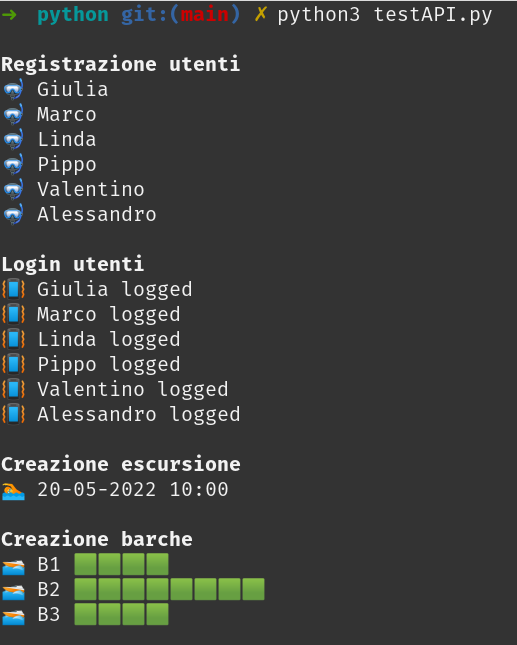
\includegraphics[width=\textwidth]{iterazione1/test/integration-test/populate-db.png}
    \centering
    \caption{Dati per Integration Test}
    \label{Dati per Integration Test}
\end{figure}

\clearpage

Una volta popolato il database di test viene testato l'algoritmo.

Vengono testati i seguenti casi:
\begin{enumerate}
    \item gruppo allocato correttamente (senza divisione gruppo) \label{caso1}
    \item gruppo non allocato (posti non terminati, ma non sufficienti per il gruppo, anche dividendolo) \label{caso2}
    \item gruppo allocato correttamente (con divisione gruppo) \label{caso3}
    \item gruppo non allocato (posti terminati)\label{caso4}
\end{enumerate}

L'esito dei test vengono mostrati in Figura \ref{Integration Test dell'algoritmo}.

\begin{figure}[htbp]
    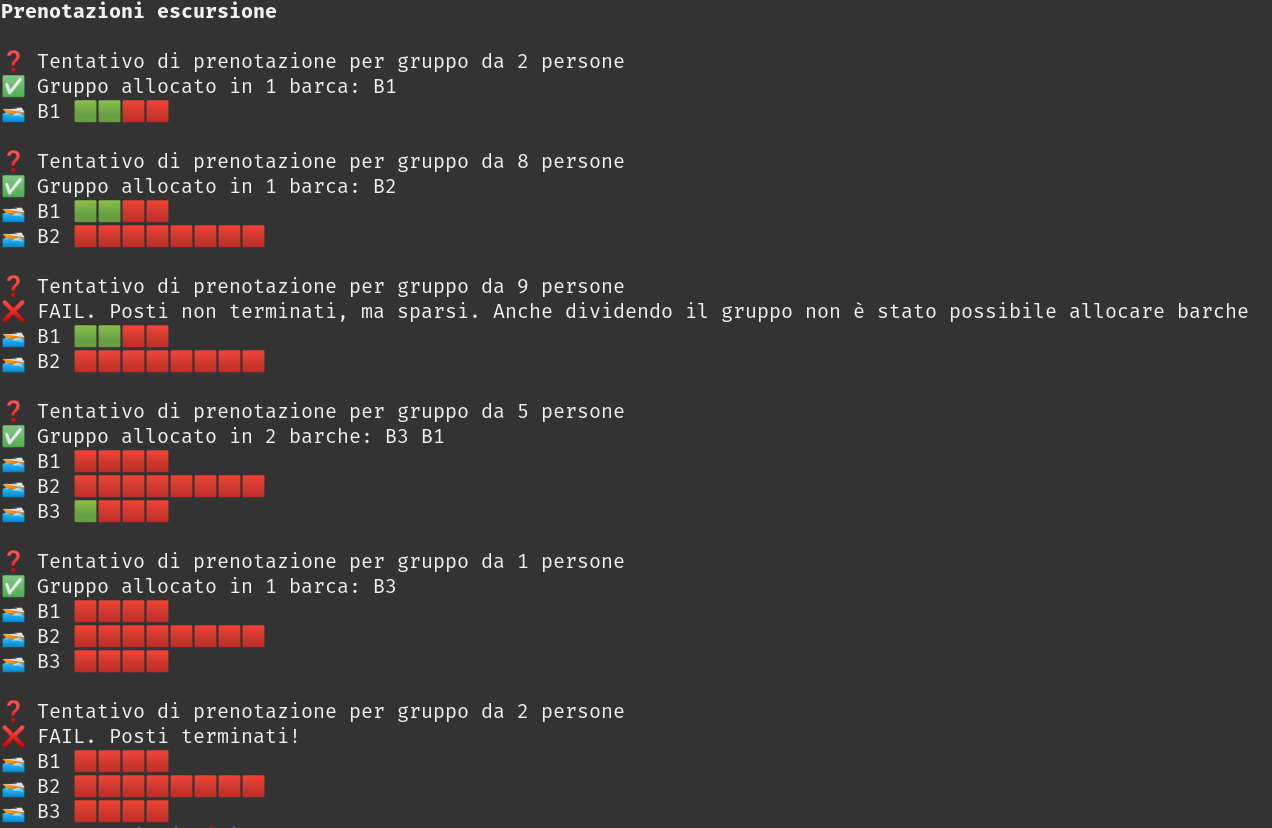
\includegraphics[width=\textwidth]{images/iterazione1/test/integration-test/bookings.png}
    \centering
    \caption{Integration Test dell'algoritmo}
    \label{Integration Test dell'algoritmo}
\end{figure}

\clearpage

L'algoritmo si comporta come previsto:
\begin{itemize}
    \item il primo, secondo e quinto tentativo di prenotazione testano il caso \ref{caso1}
    \item il terzo tentativo di prenotazione testa il caso \ref{caso2}
    \item il quarto tentativo di prenotazione testa il caso \ref{caso3}
    \item il sesto tentativo di prenotazione testa il caso \ref{caso4}.
\end{itemize}

\cleardoublepage 
\subsection{Documentazione API}
In questa sezione vengono mostrate alcune delle API sviluppate per l'iterazione 2.  
\begin{itemize}
    \item API per la realizzazione di una prenotazione. Figura \ref{API creazione prenotazione}
    \item API per la visualizzazione delle prenotazioni relative ad una escursione specifica. Figura \ref{visualizazione prenotazioni per escursione}
\end{itemize}

\begin{figure}[htbp]
    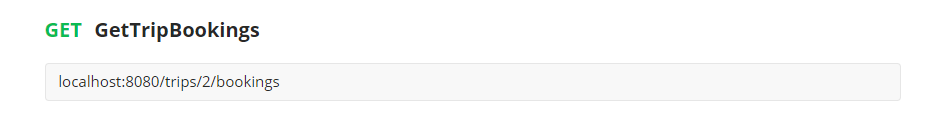
\includegraphics[width=\textwidth]{images/iterazione2/postman-api/GetTripBookings.PNG}
    \centering
    \caption{API per la creazione di una prenotazione}\label{API creazione prenotazione}
\end{figure}
\begin{figure}[htbp]
    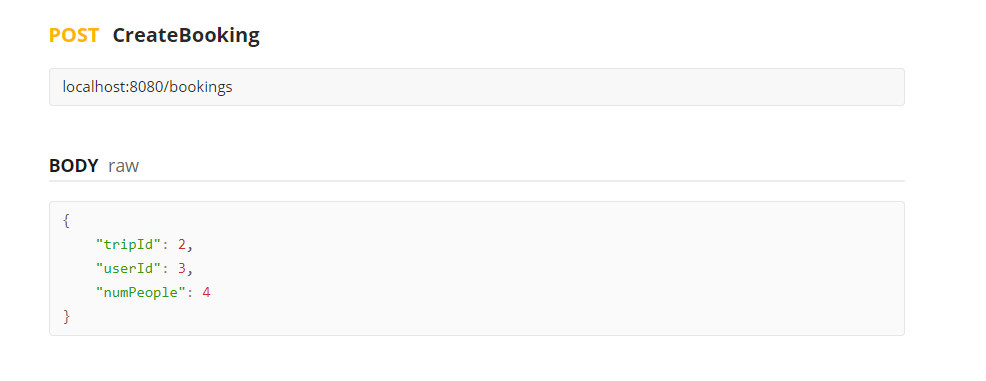
\includegraphics[width=\textwidth]{images/iterazione2/postman-api/CreateBooking.PNG}
    \centering
    \caption{API per la visualizzazione delle prenotazioni relative ad una escursione specifica}
    \label{visualizazione prenotazioni per escursione}
\end{figure}

\cleardoublepage 
